\documentclass{beamer}
\usetheme{SimplePlus}

\usepackage{hyperref}
\usepackage{graphicx}
\usepackage{booktabs}
\usepackage{subcaption}

\usepackage[backend=biber]{biblatex}

\addbibresource{references.bib}

\title{CPU Scheduling}

\author{Colby Cox}

\institute {
  University of Central Arkansas
}
\date{April 21, 2025}

\begin{document}

\begin{frame}
	\titlepage
\end{frame}

\begin{frame}{States of a Process}
	There are three states a process can be in:
	\begin{itemize}
		\item Waiting - When a process is waiting to be selected for the ready queue by the CPU scheduler.
		\item Ready - When a process will be ran on the CPU the next time a thread is available.
		\item Running - When a process is currently running on the CPU.
	\end{itemize}
\end{frame}

\begin{frame}{Algorithms Implemented}
	\begin{itemize}
		\item First Come First Served (FCFS) - The processes will be scheduled in order of arrival time.
		\item Shortest Job First (SJF) - The processes will be scheduled in order of shortest burst time.
		\item Priority - Priority scheduling is when each process is given a priority level, which determines the order of processes to be executed in.\end{itemize}
\end{frame}

\begin{frame}{Grading Criteria}
	\begin{itemize}
		\item CPU Utilization - Can range from 0 to 100 percent. Represents how busy the average thread of the CPU is.
		\item Throughput - Average number of processes that are completed per time unit.
		\item Turnaround Time - Interval of time from the submission of a process to the time of completion of a process. Sum of time spent in ready queue, execution time, and time doing I/O.
		\item Waiting Time - Sum of the periods spent in the ready queue.
		\item Response Time - The time it takes a process to start responding, rather than completing.
	\end{itemize}
\end{frame}

\begin{frame}{Our Example}
	\begin{figure}
		\begin{center}
			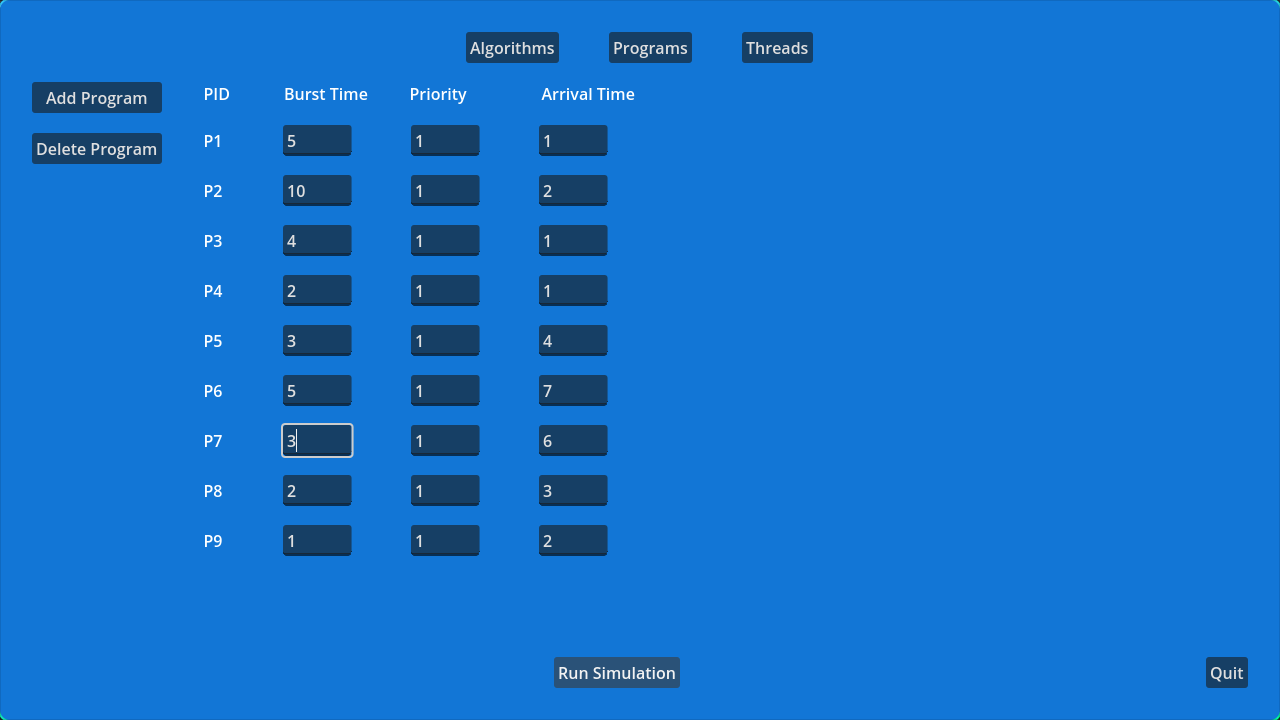
\includegraphics[width=0.95\textwidth]{Example.png}
		\end{center}
		\caption*{The example we will use with the different algorithms}
	\end{figure}
\end{frame}

\begin{frame}{Shortest Job First}
	\centering
	\begin{figure}[h!]
		\begin{subfigure}{0.9\textwidth}
			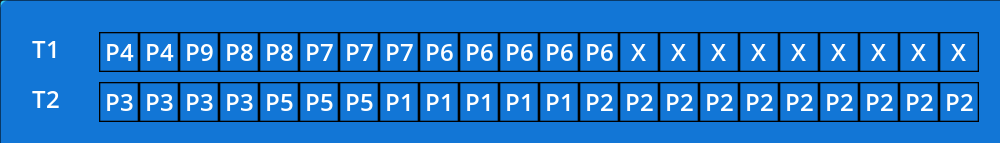
\includegraphics[width=1\textwidth]{SJFSchedule.png}
			\caption*{\large SJF's Schedule}
		\end{subfigure} \\
		\begin{subfigure}{0.6\textwidth}
			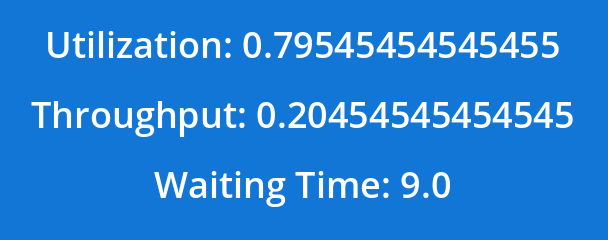
\includegraphics[width=1\textwidth]{SJFGrade.png}
			\caption*{\large SJF's Grade}
		\end{subfigure}
	\end{figure}
\end{frame}

\begin{frame}{First Come First Serve}
	\centering
	\begin{figure}[h!]
		\begin{subfigure}{0.9\textwidth}
			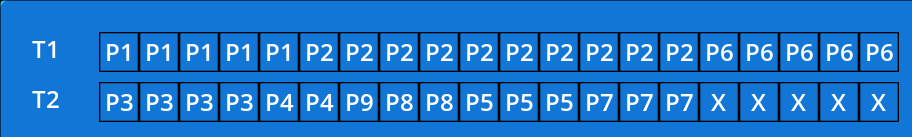
\includegraphics[width=1\textwidth]{FCFSSchedule.png}
			\caption*{\large FCFS's Schedule}
		\end{subfigure} \\
		\begin{subfigure}{0.4\textwidth}
			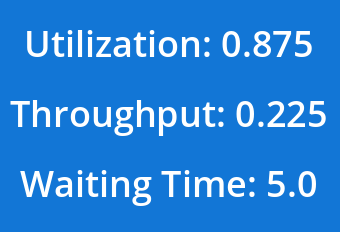
\includegraphics[width=1\textwidth]{FCFSGrade.png}
			\caption*{\large FCFS's Grade}
		\end{subfigure}
	\end{figure}
\end{frame}

\begin{frame}{SJF with Priority}
	\centering
	\begin{figure}[h!]
		\begin{subfigure}{0.9\textwidth}
			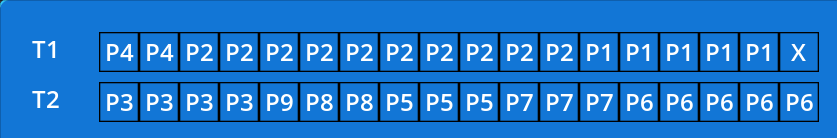
\includegraphics[width=1\textwidth]{PrioritySchedule.png}
			\caption*{\large Priority's Schedule}
		\end{subfigure} \\
		\begin{subfigure}{0.6\textwidth}
			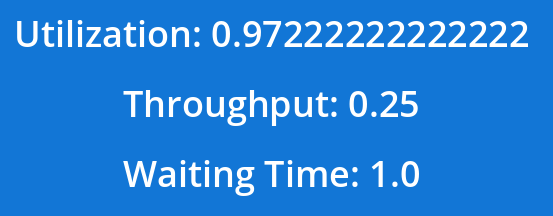
\includegraphics[width=1\textwidth]{PriorityGrade.png}
			\caption*{\large Priority's Grade}
		\end{subfigure}
	\end{figure}
\end{frame}

\begin{frame}{Future Considerations}
	\begin{itemize}
		\item Multithreading
		\item More complex algorithms like Highest Response Ratio Next and Multilevel Queue.
	\end{itemize}
\end{frame}

\begin{frame}{Conclusions}
	\begin{itemize}
		\item There is no "perfect" scheduling algorithm since it is dependent on a cpu's use case and prioritizing appropriately.
		\item Scheduling algorithms are often combinations of previous less complex algorithms.
		\item This program can be found at \underline{https://github.com/ColbysPrograms/cpuScheduling}
	\end{itemize}
\end{frame}

\begin{frame}{References}
	\nocite{*}
	\printbibliography
\end{frame}

\end{document}
